% Provenance (never printed): see sources/outline_sources.md (Year 3:
% stereographic projection; fold and fault analysis; palaeostress; balanced
% cross-sections). Brief: sources/book5/BRIEFS.md, ch. 8. Nets, pi-diagram and
% fault-slip data from figdata/bachelor-3/stereonet.py (Varden data invented,
% from figdata/shared/region.py); Fry plot from figdata/bachelor-3/fry.py.
% Exercise and problem values in the Book 5 scratch calculator calc/ch08.py.
% No real-world numbers: no ledger rows.
\chapter{التحليل البنيوي}\label{ch:b3:structural-analysis}

قاس جيولوجيّ مئتي مستوٍ طبقيّ على أجنحة طيّةٍ
أكبر من أن تُرى كاملةً: يقع مفصلها تحت غابة، وتمتدّ أجنحتها كيلومترات.
كلّ قراءة زوج من الأعداد. وعند تمثيل هذه النقاط على مخطّط دائريّ،
تقع أقطاب المستويات على منحنى واحد هو دائرة عظمى، وقطب تلك الدائرة العظمى هو
محور الطيّة، وهو خطّ لم يرَه أحدٌ قطّ.
يبني هذا الفصل المخطّط، أي \omterm{def:b3:structural-analysis:stereo}{الإسقاط الستيريوغرافي}،
ويستخدمه، مع أدوات المتجهات التي تقوم عليه، لإيجاد محاور الطيّات، ولقياس الانفعال المسجّل في
الأجسام المشوّهة، ولاستعادة الإجهاد الذي أدّى إلى مجموعة من الصدوع، ولترميم مقطع عرضيّ مشوّه
إلى حالته قبل
التشوّه.

\begin{recall}
الدوائر العظمى والصغرى للكرة واردة في مجلد السنة الأولى، في فصلها
المتعلّق بالفلك الكروي؛ والامتداد والانحدار واتجاه الانحدار والاتجاه والغوص واردة في فصليه
عن الخرائط الجيولوجية والمقاطع العرضية؛ والعمودي الواحدي الصاعد على مستوٍ
اتجاه انحداره $\alpha$ وانحداره $\delta$، $\vec n = (\sin\delta
\sin\alpha, \sin\delta\cos\alpha, \cos\delta)$ بمركّبات شرقية وشمالية وصاعدة،
ومتوسط المتجهات لمجموعة من القراءات في فصله الأول عن الطرائق الميدانية والمخبرية.
عناصر الطيّات وأصنافها، وخط مفصل الطية الموازي
للجداء $\vec n_1\times\vec n_2$ وزاوية الأجنحة
$\ang{180} - \arccos(\vec n_1\cdot\vec n_2)$، وكذلك نظرية أندرسون في تشكّل الصدوع،
واردة في فصله عن الصدوع والطيّات والنسيج؛ والإجهاد،
والإجهادات الرئيسية، والقطع الناقص للانفعال، والقصّ البسيط، في فصله عن
الإجهاد والانفعال والريولوجيا؛ وزاوية الانزلاق لمتجهة الانزلاق (انطلاقًا من الامتداد،
\ang{-90} للصدع العادي، و\ang{90} للصدع المعكوس، و0 للصدع الأيسر،
و\ang{180} للصدع الأيمن) ومحورا P وT للآلية البؤرية في فصله عن مصدر الزلزال.
والمقطع العرضي المتوازن وسطح الانفصال واردان في مجلد السنة الثانية،
في فصله عن الألب. والمربعات الصغرى واردة
في \cref{sec:b3:seismology-imaging:inverse}؛ والقيم الذاتية والمتجهات الذاتية لمصفوفة متناظرة واردة في
كتب الرياضيات.
\end{recall}

\section{الإسقاط الستيريوغرافي}\label{sec:b3:structural-analysis:stereo}

بيانات الجيولوجيّ توجّهاتٌ: وضعيةُ مستوٍ طبقيّ،
وصدعٍ، وتورّقٍ؛ واتجاهُ الغوص والاتجاهُ لتخطّطٍ، ومفصلِ طيّةٍ، واتجاهِ
الانزلاق. كلٌّ منها اتجاهٌ يمرّ بنقطة دون موضع. ولمقارنة مئات منها،
نتخيّلها جميعًا منقولةً إلى مركز كرةٍ واحدةٍ:
يلتقي الخطُّ بالنصف السفلي للكرة عند نقطة واحدة، ويقطعها المستوي وفق
نصف دائرة عظمى. ويُظهر مخطّط النصف السفلي عندئذٍ الخطوط نقاطًا،
والمستويات منحنيات.

\begin{definition}[الإسقاط الستيريوغرافي، الشبكة متساوية الزوايا، الإسقاط متساوي المساحات، القطب]\label{def:b3:structural-analysis:stereo}
ليكن خطٌّ مارًّا بمركز $O$ لكرةٍ نصف قطرها $R$، يلتقي النصف السفلي
للكرة عند $P$، بزاوية $\theta = \ang{90} - p$ عن نظير سمت الرأس، حيث
$p$ هو غوص الخط، و$t$ اتجاهه. \emph{الإسقاط
الستيريوغرافي}\index{الإسقاط الستيريوغرافي} يرسل $P$ إلى النقطة التي يتقاطع فيها
الخط المستقيم من سمت الرأس إلى $P$ يقطع المستوي الأفقي المار بالمركز
$O$؛ تقع تلك النقطة على البعد $r$ من $O$ في السمت $t$. والمخطّط الذي يمثّل النصف السفلي
مرسومًا بهذه الطريقة، ومعه شبكته من الدوائر العظمى والصغرى، هو
\emph{الشبكة متساوية الزوايا}\index{الشبكة متساوية الزوايا} (أو
شبكة وولف). و\emph{الإسقاط متساوي المساحات (للكرة)}\index{الإسقاط متساوي المساحات (للكرة)}
يرسل $P$ إلى النقطة التي تقع على البعد $r =
R\sqrt2\sin(\theta/2)$ في السمت $t$؛ وشبكته هي شبكة شميدت.
و\emph{القطب}\index{القطب (للمستوي)} لمستوٍ هو خطّه العمودي، ويُرسم
نقطةً؛ فلمستوٍ اتجاه انحداره $\alpha$ وانحداره $\delta$ يكون القطب
اتجاهه $\alpha + \ang{180}$ وغوصه $\ang{90} - \delta$.
\end{definition}

كلا الإسقاطين يضعان الخط الرأسي في المركز والخط الأفقي على
دائرة نصف قطرها $R$، وهي الدائرة الأولية. ويختلفان فيما يحفظانه.

\begin{theorem}[الإسقاطان]\label{thm:b3:structural-analysis:projections}
\begin{enumerate}[label=(\alph*)]
  \item يضع \omterm{def:b3:structural-analysis:stereo}{الإسقاط الستيريوغرافي} النقطة $P$ على البعد $r = R\tan(\theta/2)$. وهو
        تشاكليّ: عند كل نقطة يمطّ جميع الاتجاهات بالعامل نفسه،
        $1/(2\cos^2(\theta/2))$، بحيث يحفظ الزوايا بين
        المنحنيات.
  \item يضرب الإسقاط متساوي المساحات كل مساحة بالعامل نفسه،
        $1/2$: مساحة أيّ منطقة من الشبكة هي نصف مساحة المنطقة
        من نصف الكرة التي تمثّلها.
\end{enumerate}
\end{theorem}

\begin{proof}
(أ) في المستوي الرأسي المارّ بسمت الرأس $Z$ ونظير سمت الرأس والنقطة $P$
(الشكل الأول أدناه)، يقابل القوسُ الممتدّ من النظير إلى $P$ الزاويةَ $\theta$ عند المركز،
ومن ثمّ الزاوية المحيطية
$\theta/2$ عند $Z$، وهي على البعد $R$ فوق $O$: $r =
R\tan(\theta/2)$. وتصبح الخطوة الصغيرة $R\,\mathrm d\theta$ على الكرة نحو
النظير $\mathrm dr = R\,\mathrm d\theta/(2\cos^2(\theta/2))$ على
المخطّط. ودائرة النقاط ذات الزاوية $\theta$ عن النظير
محيطها $2\pi R\sin\theta$، وتصبح دائرة محيطها $2\pi
r$؛ والنسبة $\tan(\theta/2)/\sin\theta = 1/(2\cos^2(\theta/2))$، وهي نفسها
على طول نصف القطر. والخريطة التي تمطّ بالتساوي في اتجاهين متعامدين
تمطّ بالتساوي في جميع الاتجاهات، وتحفظ الزوايا.

(ب) مساحة القلنسوة الكروية ضمن الزاوية $\theta$ من النظير هي
$2\pi R^2(1 - \cos\theta) = 4\pi R^2\sin^2(\theta/2)$؛ وصورتها القرص
مساحته $\pi r^2 = 2\pi R^2\sin^2(\theta/2)$، أي نصفها. وتُوزَّع المساحتان
بالتساوي في السمت، فإنّ قطاع القلنسوة المحصور بين سمتين
وصورته يحتفظان بالنسبة $1/2$، وكذلك الحلقة المحصورة بين قيمتين
من $\theta$، وهي الفرق بين قلنسوتين. وكلّ منطقة هي اتحاد لمثل
هذه القطاعات الحلقية الصغيرة.
\end{proof}

يحوّل \omterm{def:b3:structural-analysis:stereo}{الإسقاط الستيريوغرافي} أيضًا كل دائرة من الكرة، عظمى كانت أو صغرى،
إلى دائرة أو خطّ مستقيم على المخطّط؛ ونُسلِّم بذلك. ويجعل
\omterm{def:b3:structural-analysis:stereo}{الشبكة متساوية الزوايا} سهلة الرسم بالفرجار، وتحتفظ الدائرة الصغرى، أي مخروط
الخطوط عند زاوية ثابتة عن محور، بشكلها. أمّا الإسقاط متساوي المساحات
فيشوّه الأشكال: تصبح الدائرة الصغرى بيضوية
ممطوطة حول الدائرة الأولية. وهو الإسقاط الذي يمكن عليه عدّ سحابة من الأقطاب،
لأنّ المساحات المتساوية من الشبكة تحوي حصصًا متساوية من
اتجاهات نصف الكرة؛ ويستخدمه الجيولوجيّون البنيويّون، وكذلك علماء الزلازل في
الآليات البؤرية، لبياناتهم.

\begin{omfigure}
\begin{tikzpicture}[scale=1.0, >=stealth]
% (a) equal-angle: theta = 60 deg, R = 2 cm; r = 2 tan 30 = 1.155
\begin{scope}
\draw[thick] (0,0) circle (2);
\draw (-2.5,0) -- (2.5,0) node[right, font=\scriptsize] {المستوى};
\fill (0,2) circle (1.5pt) node[above, font=\scriptsize] {\foreignlanguage{arabic}{سمت الرأس $Z$}};
\fill (0,-2) circle (1.5pt) node[below, font=\scriptsize] {نظير السمت};
\fill (0,0) circle (1.2pt) node[above left, font=\scriptsize] {$O$};
\draw[dashed] (0,2) -- (0,-2);
\draw[omDef, thick] (0,0) -- (1.732,-1);
\fill[omDef] (1.732,-1) circle (1.5pt) node[below right, font=\scriptsize] {$P$};
\draw[omThm] (0,2) -- (1.732,-1);
\fill[omThm] (1.155,0) circle (1.5pt);
\node[omThm, font=\scriptsize, above right] at (1.155,0) {$P'$};
\draw (0,-0.6) arc[start angle=-90, end angle=-30, radius=0.6];
\node[font=\scriptsize] at (0.38,-0.85) {$\theta$};
\draw (0,1.2) arc[start angle=-90, end angle=-60, radius=0.8];
\node[font=\scriptsize] at (0.25,0.95) {$\theta/2$};
\draw[<->] (0,0.25) -- (1.155,0.25);
\node[font=\scriptsize, above] at (0.58,0.25) {$r$};
\node[font=\small] at (0,-3.0) {\foreignlanguage{arabic}{(أ) الإسقاط متساوي الزوايا}};
\end{scope}
% (b) equal-area: chord from nadir to P = 2R sin(theta/2) = 2
\begin{scope}[xshift=6.6cm]
\draw[thick] (0,0) circle (2);
\draw (-2.5,0) -- (2.5,0);
\draw (-2.5,-2) -- (2.5,-2) node[right, font=\scriptsize] {المستوى المماسّ};
\fill (0,-2) circle (1.5pt) node[below left, font=\scriptsize] {نظير السمت};
\fill (0,0) circle (1.2pt) node[above left, font=\scriptsize] {$O$};
\draw[dashed] (0,2) -- (0,-2);
\draw[omDef, thick] (0,0) -- (1.732,-1);
\fill[omDef] (1.732,-1) circle (1.5pt) node[above right, font=\scriptsize] {$P$};
\draw[omThm] (0,-2) -- (1.732,-1);
\draw[omThm, dashed] (1.732,-1) arc[start angle=30, end angle=0, radius=2];
\fill[omThm] (2,-2) circle (1.5pt);
\node[omThm, font=\scriptsize, below] at (2,-2.05) {$2R\sin(\theta/2)$};
\draw (0,-0.6) arc[start angle=-90, end angle=-30, radius=0.6];
\node[font=\scriptsize] at (0.38,-0.85) {$\theta$};
\node[font=\small] at (0,-3.0) {\foreignlanguage{arabic}{(ب) الإسقاط متساوي المساحات}};
\end{scope}
\end{tikzpicture}

\par\smallskip{\small الإسقاطان في المستوى الشاقولي المار
بالخط $OP$. (أ) يرسل \omterm{def:b3:structural-analysis:stereo}{الإسقاط الستيريوغرافي} $P$ إلى $P'$، حيث يقطع
المستوى الأفقي الخطَّ الواصل من سمت الرأس: الزاوية عند $Z$ هي
$\theta/2$، فإنّ $r = R\tan(\theta/2)$. (ب) يحمل الإسقاط متساوي المساحات
$P$، حول نظير السمت، على المستوى المماسّ عند المسافة $2R\sin(\theta/2)$
من الوتر؛ ثم يُعدَّل مقياس المخطط بعامل $1/\sqrt2$ بحيث تقع الخطوط الأفقية
على دائرة أولية نصف قطرها $R$.}\label{fig:b3:structural-analysis:geometry}
\end{omfigure}

\begin{omfigure}
\begin{tikzpicture}
\begin{groupplot}[group style={group size=2 by 1, horizontal sep=0.8cm},
  width=0.5\linewidth, height=0.5\linewidth, axis equal image, hide axis,
  xmin=-1.15, xmax=1.15, ymin=-1.15, ymax=1.15, unbounded coords=jump,
  title style={font=\small}]
\nextgroupplot[title={(أ) الشبكة متساوية الزوايا (وولف)}]
% computed in figdata/bachelor-3/stereonet.py
\addplot[gray!75, very thin] table[x=x, y=y] {figdata/out/bachelor-3-stereonet-wulff.dat};
\addplot[gray!75, very thin] coordinates {(-1,0) (1,0)};
\addplot[black, thick, domain=0:360, samples=181] ({cos(x)}, {sin(x)});
\node[font=\scriptsize, above] at (axis cs:0,1.0) {\omnameCompassN};
\nextgroupplot[title={(ب) الشبكة متساوية المساحات (شميت)}]
\addplot[gray!75, very thin] table[x=x, y=y] {figdata/out/bachelor-3-stereonet-schmidt.dat};
\addplot[gray!75, very thin] coordinates {(-1,0) (1,0)};
\addplot[black, thick, domain=0:360, samples=181] ({cos(x)}, {sin(x)});
\node[font=\scriptsize, above] at (axis cs:0,1.0) {\omnameCompassN};
\end{groupplot}
\end{tikzpicture}

\par\smallskip{\small الشبكتان، مرسومتان من صيغ المبرهنة
السابقة: الدوائر العظمى للمستويات ذات الامتداد شمال--جنوب والانحدار كلّ
\ang{10} شرقًا وغربًا، والدوائر الصغرى كلّ \ang{10} حول
المحور شمال--جنوب. على \omterm{def:b3:structural-analysis:stereo}{الشبكة متساوية الزوايا} تكون الدوائر الصغرى دوائر؛ على
الشبكة متساوية المساحات تكون بيضوية، لكنّ المساحات المتساوية تحوي حصصًا متساوية من
الاتجاهات.}\label{fig:b3:structural-analysis:nets}
\end{omfigure}

\paragraph{المستويات والخطوط والزوايا.}
يقطع مستوى ذو اتجاه انحدار $\alpha$ وانحدار $\delta$ نصفَ الكرة السفلي
على نصف دائرة عظمى. تقع طرفاه على الدائرة الأولية عند طرفي
الامتداد؛ أمّا وسطه فهو خطّ أشدّ الانحدار، الذي يغوص بزاوية $\delta$
نحو $\alpha$؛ ويبعد قطبه \ang{90} عن كلّ نقطة فيه، في
السمت $\alpha + \ang{180}$. الخطّ الواقع في المستوى نقطة على
الدائرة العظمى. لتمثيل البيانات يُوضع تراكب شفّاف على الشبكة ويُدار
حول المركز حتى يقع امتداد البيانات على قطر الشبكة شمال--جنوب؛
 ثم تُرسم الدائرة العظمى للانحدار الصحيح، ويُعاد التراكب
إلى وضعه الأصلي. تُقاس الزاوية بين خطّين على طول الدائرة العظمى
المارّة بالنقطتين معًا، بعدّ تقسيمات الدوائر الصغرى التي تقطعها، بعد
تدوير التراكب حتى تقعا على دائرة عظمى واحدة في الشبكة. والزاوية
بين مستويين هي الزاوية بين قطبيهما أو مكمّلتها.
ويقوم الحاسوب بالعمل نفسه بالمتجهات: الزاوية بين خطّين لمتجهين وحدويّين
$\vec u$ و$\vec v$ هي $\arccos|\vec u\cdot\vec v|$.

\begin{method}[تدوير البيانات حول محور]\label{met:b3:structural-analysis:rotation}
لإلغاء إمالة، مثلًا لإعادة طبقة إلى الوضع الأفقي مع
التخطّطات التي تحملها، أو لاستعادة اتجاه مغنطيسي قديم مقيس في
طبقات مائلة (انظر \cref{ch:b3:palaeomagnetism}):
\begin{enumerate}
  \item اختر محور الدوران: في الطبقة المائلة، خطّ امتدادها،
        أفقيًّا؛ والزاوية هي الانحدار، في الاتجاه الذي يرفع الطبقة.
  \item على الشبكة، أدِر التراكب حتى يقع المحور على طول
        قطر الشبكة شمال--جنوب، حيث تكون الدوائر الصغرى مخاريطَ
        حوله.
  \item انقل كلّ نقطة على طول دائرتها الصغرى بمقدار زاوية الدوران،
        مقيسةً على الدوائر العظمى. النقطة التي كانت ستخرج من نصف الكرة السفلي
        تظهر من جديد عند الطرف المقابل لدائرتها الصغرى، في
        السمت المقابل.
  \item أعِد التراكب إلى وضعه. وبالمتجهات، دوران $\vec v$ بالزاوية
        $\omega$ حول المحور الوحدوي $\vec k$ هو $\vec v' = \vec v
        \cos\omega + (\vec k\times\vec v)\sin\omega + \vec k(\vec k\cdot\vec
        v)(1 - \cos\omega)$.
\end{enumerate}
\end{method}

\section{تحليل الطيّات}\label{sec:b3:structural-analysis:folds}

تتولّد الطية الأسطوانية بخطّ مستقيم هو محور الطية، يُحرَّك
موازيًا لنفسه. كلّ مستوٍ مماسّ للسطح المطويّ يحوي المحور، فكلّ عمودي على السطح يكون
عموديًا على المحور، فتقع جميع
الأقطاب على الدائرة العظمى للمستوي العمودي على المحور.

\begin{definition}[مخطط باي، محور بيتا]\label{def:b3:structural-analysis:pi}
\emph{مخطط باي}\index{مخطط باي} للطية هو رسم أقطاب
المستويات المقيسة على سطحها المطويّ. في الطية الأسطوانية تقع هذه الأقطاب على دائرة عظمى، هي
حزام $\pi$؛ وقطب الحزام هو
\emph{محور بيتا}\index{محور بيتا}، وهو تقدير محور الطية الذي تعطيه
القياسات.
\end{definition}

عند وجود جناحين فقط يكون \omterm{def:b3:structural-analysis:pi}{محور بيتا} هو الجداء الاتّجاهي لناظميهما، كما بيّن
مجلد السنة الأولى لخطّ المفصل. ومع مئتي قراءة متناثرة يلزم أفضل توفيق.
ولا يصلح المتوسّط الاتّجاهي، الذي استُعمل لقراءات مستوٍ واحد، لأنّ أقطاب الحزام
تتّجه في كلّ اتجاه على طوله، فلا يقول متوسّطها إلّا القليل
عن الدائرة التي تقع عليها.

\begin{definition}[موتّر التوجّه]\label{def:b3:structural-analysis:orientation-tensor}
\emph{موتّر التوجّه}\index{موتّر التوجّه} لعدد $N$ من المتجهات الوحدوية
$\vec p_1, \dots, \vec p_N$ هي المصفوفة المتناظرة
\[
  T = \frac1N\sum_{i=1}^N \vec p_i\,\vec p_i^{\mathsf T},
  \qquad T_{jk} = \frac1N\sum_i p_{ij}\,p_{ik} .
\]
لا يتغيّر عندما تُستبدل متجهة بمعاكستها، لذلك فهو يناسب
المحاور والأقطاب، التي لا اتجاه لها. وقيمها الذاتية $\lambda_1 \ge \lambda_2
\ge \lambda_3 \ge 0$ مجموعها يساوي أثره، أي $1$.
\end{definition}

\begin{theorem}[العنقود والحزام من موتّر التوجّه]\label{thm:b3:structural-analysis:tensor}
لأيّ متجهة وحدوية $\vec u$،
\[
  \frac1N\sum_{i=1}^N (\vec p_i\cdot\vec u)^2 = \vec u^{\mathsf T}T\,\vec u ,
\]
الذي يأخذ أصغر قيمة له، $\lambda_3$، عندما تكون $\vec u$ المتجهة الذاتية
$\vec e_3$ الموافقة لأصغر قيمة ذاتية، وأكبر قيمة له، $\lambda_1$، على امتداد
المتجهة الذاتية $\vec e_1$. وبما أنّ $\vec p_i\cdot\vec u$ هو جيب الزاوية
بين $\vec p_i$ والمستوي العمودي على $\vec u$، فإنّ الدائرة العظمى
العمودية على $\vec e_3$ هي الحزام الذي يُصغّر مجموع مربّعات
جيوب مسافات الأقطاب إليه، و$\sqrt{\lambda_3}$ هو
جذر متوسّط مربّعات الجيب. والمحور $\vec e_1$ هو الخطّ الأقرب إلى المتجهات،
أي المحور المتوسّط للعنقود.
\end{theorem}

\begin{proof}
$(\vec p_i\cdot\vec u)^2 = \vec u^{\mathsf T}\vec p_i\,\vec p_i^{\mathsf T}\vec
u$؛ نأخذ المتوسّط على $i$. المصفوفة $T$ متناظرة، فلها أساس متعامد منظَّم
من المتجهات الذاتية، يكون فيه $\vec u = \sum_k u_k\vec e_k$ مع $\sum_k
u_k^2 = 1$ و$\vec u^{\mathsf T}T\vec u = \sum_k\lambda_k u_k^2$. وهذا متوسّط
مرجّح للقيم الذاتية، بأوزان $u_k^2$ مجموعها يساوي 1: فهو
يقع بين $\lambda_3$ و$\lambda_1$، ويبلغهما عندما تكون $\vec u = \vec
e_3$ و$\vec e_1$.
\end{proof}

تصف القيم الذاتية شكل البيانات. للعنقود $\lambda_1$ قريبة من
1، والقيمتان الأخريان صغيرتان؛ وللحزام $\lambda_3$ قريبة من 0، إذ تكون الأقطاب
منتشرة على طول الدائرة بحيث تتقاسم $\lambda_1$ و$\lambda_2$ الباقي؛
والمتجهات المتناثرة بانتظام تعطي ثلاث قيم ذاتية قريبة من $1/3$. والطية
أسطوانية، ضمن دقّة القراءات، عندما يكون $\sqrt{\lambda_3}$
غير أكبر من تشتّت القراءات المكرّرة لمستوٍ واحد. والطية المخروطية،
أو طيّتان من جيلين، تُفرِّق الأقطاب عن أيّ دائرة عظمى واحدة
وترفع $\lambda_3$.

يعرض الشكل أدناه اثنتي عشرة قراءة من جناحي طية فاردن المحدّبة،
وهي الطية المختلقة للسلسلة (انظر \cref{pb:b3:structural-analysis:1}
تحسب محورها). تتجمّع أقطاب الجناحين المائلين برفق قرب مركز
الشبكة في مجموعتين، تعرّفان معًا حزامًا يمتدّ تقريبًا في اتجاه شرق–غرب،
ويقع \omterm{def:b3:structural-analysis:pi}{محور بيتا} على الدائرة الأولية، قريبًا من الشمال تمامًا. والمستويات
المتوسّطة للجناحين، المرسومة دوائر عظمى، تتقاطع عند النقطة نفسها:
\omterm{def:b3:structural-analysis:pi}{محور بيتا} هو الخطّ المشترك لكلّ الأجنحة.

\begin{omfigure}
\begin{tikzpicture}
\begin{groupplot}[group style={group size=2 by 1, horizontal sep=1.0cm},
  width=0.5\linewidth, height=0.5\linewidth, axis equal image,
  unbounded coords=jump, title style={font=\small}]
\nextgroupplot[hide axis, xmin=-1.15, xmax=1.15, ymin=-1.15, ymax=1.15,
  title={(أ) النصف السفلي}]
% computed in figdata/bachelor-3/stereonet.py (Varden readings invented)
\addplot[gray!35, very thin] table[x=x, y=y] {figdata/out/bachelor-3-stereonet-schmidt.dat};
\addplot[black, thick, domain=0:360, samples=181] ({cos(x)}, {sin(x)});
\addplot[gray, densely dashed] table[x=x, y=y] {figdata/out/bachelor-3-stereonet-limbs.dat};
\addplot[omDef, thick] table[x=x, y=y] {figdata/out/bachelor-3-stereonet-girdle.dat};
\addplot[only marks, mark=*, mark size=1.2pt] table[x=x, y=y] {figdata/out/bachelor-3-stereonet-poles.dat};
\addplot[only marks, mark=triangle*, mark size=3pt, omThm] table[x=x, y=y] {figdata/out/bachelor-3-stereonet-beta.dat};
\node[font=\scriptsize, above] at (axis cs:0,1.02) {\omnameCompassN};
\node[omThm, font=\scriptsize, right] at (axis cs:0.06,0.88) {$\beta$};
\draw[gray] (axis cs:-0.3,-0.3) rectangle (axis cs:0.3,0.3);
\nextgroupplot[xmin=-0.3, xmax=0.3, ymin=-0.3, ymax=0.3, title={(ب) المركز مكبّرًا},
  xtick=\empty, ytick=\empty]
\addplot[gray!35, very thin] table[x=x, y=y] {figdata/out/bachelor-3-stereonet-schmidt.dat};
\addplot[omDef, thick] table[x=x, y=y] {figdata/out/bachelor-3-stereonet-girdle.dat};
\addplot[only marks, mark=*, mark size=1.5pt] table[x=x, y=y] {figdata/out/bachelor-3-stereonet-poles.dat};
\node[font=\scriptsize, align=center] at (axis cs:0.16,0.09) {أقطاب\\ الجناح الغربي};
\node[font=\scriptsize, align=center] at (axis cs:-0.16,0.09) {أقطاب\\ الجناح الشرقي};
\node[omDef, font=\scriptsize] at (axis cs:0.17,-0.06) {\foreignlanguage{arabic}{حزام \mbox{\textdir TLT $\pi$}}};
\end{groupplot}
\end{tikzpicture}

\par\smallskip{\small \omterm{def:b3:structural-analysis:pi}{مخطط باي} لطية فاردن المحدّبة على الشبكة متساوية
المساحات، النصف السفلي: أقطاب اثنتي عشرة قراءة للطبقية (نقاط)،
الحزام الأفضل توفيقًا المستخرَج من \omterm{def:b3:structural-analysis:orientation-tensor}{موتّر التوجّه} (أزرق)، والدوائر العظمى
للجناحين المتوسّطين (متقطّعة) \omterm{def:b3:structural-analysis:pi}{ومحور بيتا} (مثلّث)، حيث تتلاقى الدوائر الثلاث
جميعها. طبقة تميل شرقًا يقع قطبها إلى غرب
المركز.}\label{fig:b3:structural-analysis:pi}
\end{omfigure}

\section{تحليل الانفعال المحدود}\label{sec:b3:structural-analysis:strain}

تسجّل الصخرة المشوَّهة انفعالها حين تحتوي على أجسام يُعرف شكلها الأصلي أو ترتيبها الأصلي، مثل
الأويدات الكروية وبقع الاختزال، وأحافير معلومة التناظر، والحصى،
أو ببساطة مراكز الحبيبات التي كانت متباعدة بالتساوي
ذات يوم.

\begin{definition}[تحليل الانفعال المحدود، طريقة فراي]\label{def:b3:structural-analysis:strain-analysis}
\emph{تحليل الانفعال المحدود}\index{تحليل الانفعال المحدود} هو قياس
القطع الناقص للانفعال، أو الإهليلجي الانفعالي، الذي تعرّضت له الصخرة، انطلاقًا من أشكال
الأجسام واتجاهاتها وتباعداتها، وهي أجسام تُعرف حالتها قبل
التشوّه. وفي \emph{طريقة فراي}\index{طريقة فراي}، يُرسم المتجه
من مركز كل جسم إلى مركز كل جسم آخر، من أصل مشترك واحد؛
وإذا كانت المراكز موزّعة بحدّ أدنى للتباعد وبلا اتجاه مفضّل،
فإنّ المنطقة الخالية حول الأصل تكون قطعًا ناقصًا يماثل شكل القطع الناقص للانفعال
واتجاهه.
\end{definition}

\begin{proposition}[الفراغ في مخطط فراي]\label{prop:b3:structural-analysis:fry}
إذا حوّل انفعال متجانس كلّ متجه $\vec d$ إلى $F\vec d$، ولم تكن أيّ مركزين
أقرب من $d_0$ قبل الانفعال، فإنّ المنطقة بعده حول أصل مخطط فراي
الخالية من النقاط تحوي القطع الناقص
$\{F\vec d : |\vec d| < d_0\}$، ذا نصفَي المحورين $S_1d_0$ و$S_2d_0$ على امتداد
الاتجاهات الرئيسية للانفعال.
\end{proposition}

\begin{proof}
ينقل الانفعال المتجانس كل نقطة بالتحويل الخطّي نفسه، مضافًا إليه
انسحاب، فيصبح فرق مركزين هو $F\vec d$. قبل الانفعال لم يقع أيّ فرق
في القرص الذي نصف قطره $d_0$؛ وبعده لا يقع أيّ فرق في صورته،
وهي القطع الناقص للانفعال من مجلد السنة الأولى مضروبًا في $d_0$.
\end{proof}

عمليًّا لا تكون المراكز كلها على الحدّ الأدنى للتباعد، ويُقرأ الفراغ
بوصفه الحافة الداخلية لأكثف حلقة من النقاط، وتُقدَّر نسبته
نسبة الانفعال $R_s = S_1/S_2$ بقيمة أدنى قليلًا. يُجري الشكل الآتي الاختبار
على شريحة رقيقة مُتخيَّلة، مشوَّهة حتى $R_s = 2$ مع امتداد المحور الطويل عند
\ang{30} عن الأفقي: القطع الناقص الملائم لحافة الفراغ يعطي
$R_s = 1.9$ و\ang{30}. وعند قياس الأجسام نفسها، تصبح الأجسام المستديرة في البداية
قطعًا ناقصة نسبة محوريّها $R_s$ بالضبط؛ أمّا الأجسام الإهليلجية في البداية،
ذات الاتجاهات العشوائية، فتنتهي بنسب $R_f$ متفرّقة
حول $R_s$، وأكبرها حين تكون محاورها الطويلة في الأصل موازية
لاتجاه الاستطالة، وتتجمّع اتجاهاتها النهائية $\varphi$ حول
ذلك الاتجاه. ويفصل مخطط $R_f$ مقابل $\varphi$، المقروء بالجداول أو بالحاسوب،
الانفعال عن الأشكال الأصلية.

\begin{omfigure}
\begin{tikzpicture}
\begin{groupplot}[group style={group size=2 by 1, horizontal sep=1.2cm},
  width=0.5\linewidth, height=0.5\linewidth, axis equal image,
  title style={font=\small}, tick label style={font=\scriptsize}]
\nextgroupplot[xmin=-10, xmax=10, ymin=-10, ymax=10, title={(أ) مراكز الحبيبات بعد الانفعال}]
% computed in figdata/bachelor-3/fry.py (invented population)
\addplot[only marks, mark=o, mark size=1.6pt, black] table[x=x, y=y] {figdata/out/bachelor-3-fry-points.dat};
\nextgroupplot[xmin=-2.6, xmax=2.6, ymin=-2.6, ymax=2.6, title={(ب) مخطط فراي}]
\addplot[only marks, mark=*, mark size=0.5pt, black] table[x=x, y=y] {figdata/out/bachelor-3-fry-fry.dat};
\addplot[omThm, thick] table[x=x, y=y] {figdata/out/bachelor-3-fry-fit.dat};
\end{groupplot}
\end{tikzpicture}

\par\smallskip{\small \omterm{def:b3:structural-analysis:strain-analysis}{طريقة فراي} على مجموعة مُتخيَّلة من مراكز الحبيبات،
موزَّعة بحدّ أدنى للتباعد 1، ثم شُوِّهت حتى $R_s = 2$،
مع امتداد المحور الطويل عند \ang{30} عكس عقارب الساعة عن الأفقي، مع الحفاظ على المساحة. (أ) المراكز،
التي لا تكاد العين تلمح فيها الانفعال. (ب) المتجهات بين كل أزواج المراكز الأقرب من 2.6:
الفراغ في المركز هو القطع الناقص للانفعال. والقطع الناقص الأحمر
الملائم لأقرب نقطة في كل قطاع من 36 قطاعًا: نسبته 1.9،
والمحور الطويل عند \ang{30}.}\label{fig:b3:structural-analysis:fry}
\end{omfigure}

في ثلاثة أبعاد، للإهليلجي الانفعالي استطالات رئيسية $X \ge Y
\ge Z$. يُرسم شكله على مخطط فلين، بحيث يكون $a = X/Y$ مقابل $b =
Y/Z$ والمعامل
\[
  k = \frac{a - 1}{b - 1} .
\]
على المستقيم $k = 1$، الذي يمثّل الانفعال المستوي بحجم ثابت ($Y = 1$،
$X = 1/Z$، أي $a = b$)، لا يكون الإهليلجي سيجاريَّ الشكل ولا فطيريَّ الشكل. وفوقه،
$k > 1$، يكون الإهليلجي مستطيلًا مَطوطًا في اتجاه واحد بفعل
التضيّق: تنمو في الصخور المشوَّهة بهذه الطريقة تخطّطات قوية. وتحته، $k < 1$،
يكون مُفلطحًا، وتنمو فيه تورّقات قوية.

\begin{omfigure}
\begin{tikzpicture}[scale=1.0, >=stealth]
\draw[->] (0,0) -- (5.4,0) node[right, font=\scriptsize] {$b = Y/Z$};
\draw[->] (0,0) -- (0,4.6) node[above, font=\scriptsize] {$a = X/Y$};
\foreach \v/\l in {0/1, 1.5/2, 3/3, 4.5/4} {
  \draw (\v,0) -- (\v,-0.08) node[below, font=\scriptsize] {\l};
  \draw (0,\v) -- (-0.08,\v) node[left, font=\scriptsize] {\l};
}
\draw[omDef, thick] (0,0) -- (4.5,4.5) node[right, font=\scriptsize, align=left] {\foreignlanguage{arabic}{$k = 1$}\\\foreignlanguage{arabic}{انفعال مستوٍ}};
\node[font=\scriptsize, align=center] at (1.3,3.6) {\foreignlanguage{arabic}{التضيّق}\\\foreignlanguage{arabic}{\mbox{\textdir TLT $k > 1$}، مستطيل}};
\node[font=\scriptsize, align=center] at (4.3,1.1) {\foreignlanguage{arabic}{التفلطح}\\\foreignlanguage{arabic}{\mbox{\textdir TLT $k < 1$}، مفلطح}};
% shapes
\draw[fill=omLithLime] (0.9,2.75) ellipse (0.55 and 0.12);
\draw[fill=omLithLime] (4.3,2.1) ellipse (0.45 and 0.22);
\end{tikzpicture}

\par\smallskip{\small مخطط فلين للإهليلجيات الانفعالية. الحالة غير المشوَّهة
هي الأصل، $a = b = 1$؛ الإهليلجيات السيجارية الشكل الناتجة عن التضيّق
تقع باتجاه المحور الرأسي، والإهليلجيات الفطيرية الشكل الناتجة عن التفلطح باتجاه
المحور الأفقي.}\label{fig:b3:structural-analysis:flinn}
\end{omfigure}

\section{الإجهاد القديم}\label{sec:b3:structural-analysis:palaeostress}

تحدّد نظرية أندرسون المستويات التي تتكوّن عليها الصدوع الجديدة، وتبيّن أنّها تنزلق
عموديًّا على $\sigma_2$. غير أنّ معظم الصدوع نقاط ضعف أقدم
أُعيد تنشيطها في حقل إجهاد لم تختره، وتنزلق
انزلاقًا مائلًا. وتبقى اتجاهات انزلاقها، المقروءة على الخطوط المحزوزة في أسطح الصدوع،
تسجّل الإجهاد، شريطة أن ينزلق كل صدع بالطريقة التي
يدفعه الإجهاد بها.

\begin{definition}[الإجهاد القديم، فرضية والاس--بوت، نسبة الإجهاد، قلب انزلاق الصدوع]\label{def:b3:structural-analysis:palaeostress}
\emph{الإجهاد القديم}\index{الإجهاد القديم} هو حالة الإجهاد التي أثّرت في
صخرٍ في الماضي، بقدر ما يمكن استنتاجه من البنى التي خلّفتها:
عمليًّا، اتجاهات الإجهادات الرئيسية
و\emph{نسبة الإجهاد}\index{نسبة الإجهاد}
\[
  \Phi = \frac{\sigma_2 - \sigma_3}{\sigma_1 - \sigma_3}, \qquad 0 \le \Phi
  \le 1 .
\]
\emph{فرضية والاس--بوت}\index{فرضية والاس--بوت} تنصّ
على أنّ الصدع ينزلق موازيًا لإجهاد القصّ المحلَّل على مستواه بواسطة إجهاد
منتظم، كلّ صدع على حدة. \emph{انعكاس انزلاق
الصدوع}\index{قلب انزلاق الصدوع} هو البحث عن الاتجاهات الرئيسية
ونسبة الإجهاد التي تطابق اتجاهات الانزلاق المتنبَّأ بها أفضل مطابقة لمجموعة
من الصدوع والخطوط المحزوزة المقاسة.
\end{definition}

\begin{theorem}[اتجاه الانزلاق على مستوى]\label{thm:b3:structural-analysis:wallace-bott}
ليكن $S$ موتّر الإجهاد، والانضغاطات تُعَدّ موجبة، و$\vec n$ هو
العمودي الواحدي الصاعد على صدعٍ. نكتب
\[
  \vec\tau = S\vec n - (\vec n\cdot S\vec n)\,\vec n .
\]
وفق \omterm{def:b3:structural-analysis:palaeostress}{فرضية والاس--بوت} ينزلق الجدار المعلّق بالنسبة إلى
الجدار المرتكز على امتداد $-\vec\tau$، أي جهد القصّ الذي يمارسه
على الجدار المرتكز. وفضلًا عن ذلك:
\begin{enumerate}[label=(\alph*)]
  \item لا يتغيّر اتجاه $\vec\tau$ عند استبدال $S$ بالعبارة $aS +
        bI$ مع $a > 0$؛ ومنه لا يتعلّق إلّا بالاتجاهات الرئيسية
        وبقيمة $\Phi$، والموتّر المختزل $S' =
        \mathrm{diag}(1, \Phi, 0)$ في الإطار الرئيسي $(\vec e_1, \vec
        e_2, \vec e_3)$ يتنبّأ بالانزلاق نفسه الذي يعطيه $S$؛
  \item إذا كان $\vec n$ عموديًّا على أحد الاتجاهات الرئيسية، فإنّ الانزلاق
        عموديًّا عليه أيضًا؛
  \item مع $n_k = \vec n\cdot\vec e_k$، يكون الاتجاه هو اتجاه $\vec\tau'
        = \vec\tau_0 + \Phi\,\vec\tau_1$، وهو خطّي في $\Phi$، حيث $\vec\tau_0
        = n_1(\vec e_1 - n_1\vec n)$ و$\vec\tau_1 = n_2(\vec e_2 - n_2\vec
        n)$.
\end{enumerate}
\end{theorem}

\begin{proof}
مع اعتبار الانضغاطات موجبة، يدفع الجدار المعلّق على الجدار المرتكز، عبر
المستوى الذي عموديّه $\vec n$ والمتّجه نحو الجدار المعلّق، بالجهد
$-S\vec n$؛ جزؤه على المستوى هو $-\vec\tau$. وعندما
ينزلق الصدع يتحرّك الجدار المعلّق بالطريقة التي يجرّ بها الجدار المرتكز على امتداد
$-\vec\tau$. (تحقّق: مع $\sigma_1$ رأسيًّا، $S = \sigma_1\vec e_z\vec
e_z^{\mathsf T}$ و$-\vec\tau = -\sigma_1\cos\delta\,(\vec e_z -
\cos\delta\,\vec n)$ يشير نحو أسفل الانحدار: صدع عادي.)
(أ) $(aS + bI)\vec n - (\vec n\cdot(aS + bI)\vec n)\vec n = a\vec\tau + b(\vec
n - \vec n) = a\vec\tau$. بكتابة $\sigma_k = \sigma_3 + (\sigma_1 -
\sigma_3)s_k$ مع $s = (1, \Phi, 0)$ نجد $S = \sigma_3 I + (\sigma_1 -
\sigma_3)S'$.
(ب) $S\vec n = \sum_k\sigma_kn_k\vec e_k$؛ إذا كان $n_j = 0$، فلا يكون لكلٍّ من $S\vec n$
و$\vec n$ مركّبةٌ على $\vec e_j$، ولا $\vec\tau$.
(ج) $S'\vec n = n_1\vec e_1 + \Phi n_2\vec e_2$ و$\vec n\cdot S'\vec n =
n_1^2 + \Phi n_2^2$؛ اجمع الحدود التي تحوي $\Phi$ والتي لا تحويه.
\end{proof}

الجزء (ب) هو حالة أندرسون: صدعٌ يحوي $\sigma_2$ ينزلق
عموديًّا عليه، مهما تكن $\Phi$، فلا يُخبرنا شيئًا عن \omterm{def:b3:structural-analysis:palaeostress}{نسبة
الإجهاد}. الجزء (ج) يحوّل الانزلاق المقاس إلى $\Phi$. ليكن $\vec u$ المتّجه الواحدي
لانزلاق الجدار المعلّق، المأخوذ من زاوية الانزلاق، و$\vec w = \vec n\times\vec
u$ هو الاتجاه في المستوى العمودي عليه. ويكون الانزلاق المتنبَّأ به
موازيًا للمتّجه $\vec u$ عندما $(\vec\tau_0 + \Phi\vec\tau_1)\cdot\vec w = 0$،
وبما أنّ $\vec n\cdot\vec w = 0$،
\[
  \Phi = -\frac{n_1\,(\vec e_1\cdot\vec w)}{n_2\,(\vec e_2\cdot\vec w)} ,
\]
بشرط أن يشير الانزلاق المتنبَّأ به عندئذٍ على امتداد $+\vec u$ لا على $-\vec u$.

عندما تكون الاتجاهات الرئيسية غير معلومة، يعطي كلّ صدع معادلةً واحدة،
هي زاوية انزلاقه داخل مستواه، لأربعة مجاهيل: ثلاث زوايا توجّه
المحاور الرئيسية، و$\Phi$. وأدنى عدد هو أربعة صدوع ذات وضعيات مختلفة،
والمعتاد بضعُ عشرات. ويُصغِّر القلبُ مجموعَ
مربّعات الزوايا بين الانزلاقات المقاسة والمتنبَّأ بها، بطريقة المربعات الصغرى
على شبكة أو بالتكرار كما في \cref{sec:b3:seismology-imaging:inverse}.
تُشكّل الصدوع التي لا تتطابق مجموعةً ثانيةً، ربّما من عمر آخر.

يُظهر الشكل أدناه خمسة صدوع في تلال فاردن: الصدع العادي الرئيسي
وأربعةً أصغر، جميعها ذات انزلاق عادي. يُجرى بحثٌ شبكيّ على قيم $\Phi$
واتجاه $\sigma_3$، مع $\sigma_1$ رأسيًّا، يطابق الصدوع الخمسة جميعها ضمن ربع
درجة، مع $\sigma_3$ أفقيًّا نحو \ang{120}.

\begin{omfigure}
\begin{tikzpicture}
\begin{axis}[width=0.56\linewidth, height=0.56\linewidth, axis equal image,
  hide axis, xmin=-1.15, xmax=1.15, ymin=-1.15, ymax=1.15, unbounded coords=jump]
% computed in figdata/bachelor-3/stereonet.py (Varden faults invented)
\addplot[gray!35, very thin] table[x=x, y=y] {figdata/out/bachelor-3-stereonet-schmidt.dat};
\addplot[black, thick, domain=0:360, samples=181] ({cos(x)}, {sin(x)});
\addplot[omDef, thick] table[x=x, y=y] {figdata/out/bachelor-3-stereonet-faults.dat};
\addplot[only marks, mark=*, mark size=1.8pt, omDef] table[x=x, y=y] {figdata/out/bachelor-3-stereonet-slips.dat};
\addplot[only marks, mark=square*, mark size=2.6pt, omThm] table[x=x, y=y] {figdata/out/bachelor-3-stereonet-s1.dat};
\addplot[only marks, mark=diamond*, mark size=3pt, omProp] table[x=x, y=y] {figdata/out/bachelor-3-stereonet-s2.dat};
\addplot[only marks, mark=triangle*, mark size=3pt, omMeth] table[x=x, y=y] {figdata/out/bachelor-3-stereonet-s3.dat};
\node[font=\scriptsize, above] at (axis cs:0,1.02) {\omnameCompassN};
\node[omThm, font=\scriptsize, above left] at (axis cs:0,0) {$\sigma_1$};
\node[omProp, font=\scriptsize, above right] at (axis cs:0.5,0.87) {$\sigma_2$};
\node[omMeth, font=\scriptsize, below right] at (axis cs:0.87,-0.5) {$\sigma_3$};
\end{axis}
\end{tikzpicture}

\par\smallskip{\small بيانات انزلاق الصدوع في تلال فاردن على
الشبكة متساوية المساحات، النصف السفلي: خمسة مستويات صدعية (الدوائر العظمى) مع اتجاه انزلاق
كلّ جدار معلّق (نقاط)، والإجهادات الرئيسية للإجهاد
الأكثر مطابقةً: $\sigma_1$ رأسيًّا (مربّع)، $\sigma_2$ و$\sigma_3$
أفقيّان (معيّنات ومثلّثات، عند طرفي كلّ محور). الصدع الرئيسي،
المنحدر بزاوية \ang{60} نحو \ang{120}، يحوي $\sigma_2$ وينزلق
مباشرةً إلى أسفل انحداره؛ أمّا الصدوع الأخرى فتنزلق
مائلًا.}\label{fig:b3:structural-analysis:faults}
\end{omfigure}

محورا P وT من مجلد السنة الأولى ليسا الإجهادات الرئيسية. إنّهما
تُبنيان من مستوى الصدع والانزلاق وحدهما، بزاوية \ang{45} عن المستوى في
المستوى الذي يحوي الانزلاق والعمودي؛ صدعٌ جديد، في صخر زاوية احتكاكه قرابة
\ang{30}، يصنع نحو \ang{30} مع $\sigma_1$، وصدعٌ أُعيد تنشيطه يصنع أيّ زاوية.
آلية واحدة تُعطي محوري P وT، ولا يُعطي الإجهادَ إلّا صدوعٌ كثيرة
ذات وضعيات مختلفة تُعكس معًا.
الفرضية نفسها لها حدود: قد يتغيّر الإجهاد من صدع إلى آخر، وقد
تدور الكتل، والصدوع المتلاقية تُعيق انزلاق بعضها بعضًا.

\section{ترميم مقطع عرضي}\label{sec:b3:structural-analysis:restoration}

المقطع العرضي تفسيرٌ: بين السطح وثقوب الحفر،
يرسم الجيولوجيّ ما هو مرجَّح. ويُسمّي مجلدُ السنة الثانية، في فصله عن الألب،
المقطعَ متوازنًا حين يمكن إرجاعه إلى حالة غير مشوّهة
مع حفظ أطوال الطبقات ومساحات الوحدات، وتتجذّر الطيّات والصدوع
الزاحفة على سطح الانفصال. والترميم هو الاختبار.

\begin{definition}[ترميم المقطع، خط التثبيت، طريقة الأشرطة المنثنية]\label{def:b3:structural-analysis:restoration}
\emph{ترميم المقطع}\index{ترميم المقطع} يُلغي، على
مقطع عرضيّ مرسوم موازيًا لاتجاه النقل التكتوني، التشوّه الذي يُظهره،
حدثًا بعد حدث وبالترتيب العكسي، مع حفظ
أطوال الطبقات ومساحات الوحدات في مستوى المقطع.
\emph{خط التثبيت}\index{خط التثبيت} خطٌّ يعبر الطبقات، يُوضع حيث لم تنزلق
إحداها على الأخرى (في المقدّمة غير المشوّهة، أو على السطح المحوري لطيّة متناظرة)،
ويُعدّ عموديًّا على الطبقات في المقطع المُرجَع،
وتُقاس الأطوال انطلاقًا منه. وفي \emph{طريقة الأشرطة المنثنية}\index{طريقة الأشرطة المنثنية} تُرسم الطيّات أجنحةً مستقيمةً
بسماكة طبقة ثابتة، موصولةً عند مفاصل حادّة، يُنصِّف سطحُها المحوري
الزاويةَ بين الأجنحة؛ فتصبح كلّ طبقة خطًّا منكسرًا،
يساوي طولُها
مجموعَ قطعها المستقيمة.
\end{definition}

طبقةٌ مطويّة إلى أجنحةٍ مستقيمةٍ تنحدر بمقدار $\delta$ في أيّ من الاتجاهين، على
المسافة الأفقية $L$، يبلغ طولها $L/\cos\delta$، ويكون تقصيرها
$S = L(1/\cos\delta - 1)$، والتغيّر النسبي للطول $\cos\delta - 1$.
وتعطي المساحات النصف الآخر من الموازنة.

\begin{proposition}[العمق حتى الانفصال]\label{prop:b3:structural-analysis:detachment}
ولتكن طبقةٌ على ارتفاع $h$ فوق انفصالٍ أفقيّ، قُصِرت بمقدار $S$
في مستوى المقطع، ولْيحفظ الصخرُ الواقع بينها وبين الانفصالِ مساحتَه،
دون أن تعبر أيّ مادّة طرفي المقطع. عندئذٍ
تحقّق المساحةُ $A$ التي تعلو بها الطبقةُ المطويّة مستواها الأصلي
\[
  A = S\,h , \qquad\text{أي أنّ}\qquad h = \frac AS .
\]
\end{proposition}

\begin{proof}
قبل التشوّه كان الصخر الواقع تحت الطبقة يشغل $L_0 h$ على
طول $L_0$. وبعد التشوّه يقع الصخرُ نفسُه على طول $L_0 - S$، تحت
الطبقة، التي تقف عند المستوى الأصلي مضافًا إليه الرفعُ: مساحتُه
$(L_0 - S)h + A$. بمساواة المساحتين نجد $A = Sh$.
\end{proof}

تعطي طبقتان المجهولين كليهما: تختلف مساحتاهما الفائضتان بمقدار $S$ مضروبًا في
المسافة الرأسية بينهما. يوضّح الشكل أدناه البناء.

\begin{omfigure}
\begin{tikzpicture}[scale=1.0, >=stealth]
% (a) kink-band anticline over a detachment, drawn to balance: limbs 50 deg
% (tan 1.19175, 1/cos 1.55572), half-wavelength 2 -> rise 2.3835; S = 4/cos50 - 4
% = 2.2229, A = 4.767, h = A/S = 2.1445; competent layers 0.3 thick (0.4667
% vertically on the limbs); weak layer restored 1.5445 thick (areas 9.611 both)
\begin{scope}
\fill[omLithEvap] (0,0) -- (4,0) -- (4,1.2111) -- (2,3.5946) -- (0,1.2111) -- cycle;
\fill[omLithSand] (0,1.2111) -- (2,3.5946) -- (4,1.2111) -- (4,1.6778) -- (2,4.0613) -- (0,1.6778) -- cycle;
\fill[omLithLime] (0,1.6778) -- (2,4.0613) -- (4,1.6778) -- (4,2.1445) -- (2,4.528) -- (0,2.1445) -- cycle;
\draw (0,1.2111) -- (2,3.5946) -- (4,1.2111);
\draw (0,1.6778) -- (2,4.0613) -- (4,1.6778);
\draw[thick] (0,2.1445) -- (2,4.528) -- (4,2.1445);
\fill[pattern=north east lines, pattern color=omThm] (0,2.1445) -- (2,4.528) -- (4,2.1445) -- cycle;
\draw[omThm, dashed] (0,2.1445) -- (4,2.1445);
\node[omThm, font=\small, fill=white, inner sep=1.5pt] at (1.25,2.5) {$A$};
\draw[very thick] (-0.3,0) -- (4.3,0);
\draw[dashed, gray] (2,0) -- (2,4.8) node[above, font=\scriptsize, black] {السطح المحوري};
\draw[omMeth, very thick] (0,0) -- (0,2.1445) node[above left, font=\scriptsize] {تثبيت};
\draw[omMeth, very thick] (4,0) -- (4,2.1445) node[above right, font=\scriptsize] {تثبيت};
\draw[<->] (-0.35,0) -- (-0.35,2.1445) node[midway, left, font=\scriptsize] {$h$};
\draw[<->] (0,-0.35) -- (4,-0.35) node[midway, below, font=\scriptsize] {$L_0 - S$};
\node[font=\small] at (2,-1.0) {\foreignlanguage{arabic}{(أ) مشوَّه}};
\end{scope}
% (b) restored: length 4/cos 50 = 6.2229
\begin{scope}[xshift=5.6cm]
\fill[omLithEvap] (0,0) rectangle (6.2229,1.5445);
\fill[omLithSand] (0,1.5445) rectangle (6.2229,1.8445);
\fill[omLithLime] (0,1.8445) rectangle (6.2229,2.1445);
\draw (0,1.5445) -- (6.2229,1.5445);
\draw (0,1.8445) -- (6.2229,1.8445);
\draw[thick] (0,2.1445) -- (6.2229,2.1445);
\draw[very thick] (-0.3,0) -- (6.5,0);
\node[font=\scriptsize, above left] at (6.2229,0) {الانفصال};
\draw[omMeth, very thick] (0,0) -- (0,2.1445) node[above, font=\scriptsize] {تثبيت};
\draw[omMeth, very thick] (6.2229,0) -- (6.2229,2.1445) node[above, font=\scriptsize] {تثبيت};
\draw[dashed] (4,0) -- (4,2.9);
\draw[<->] (4,2.75) -- (6.2229,2.75) node[midway, above, font=\scriptsize] {$S$};
\draw[<->] (0,-0.35) -- (6.2229,-0.35) node[midway, below, font=\scriptsize] {$L_0$};
\node[font=\small] at (3.1,-1.0) {\foreignlanguage{arabic}{(ب) مُرجَع}};
\end{scope}
\end{tikzpicture}

\par\smallskip{\small ترميمُ طيّةٍ \omterm{def:b3:structural-analysis:restoration}{بطريقة الأشرطة المنثنية}، مرسومةٍ لتحقيق التوازن، بأجنحةٍ
عند \ang{50}. (أ) طبقتان صلبتان مطويّتان إلى أجنحة مستقيمة ذات سماكة ثابتة،
فوق طبقة ضعيفة تزداد سماكتها لتشكّل اللبّ، بين خطّي تثبيت
على السطحين المحوريين للطيّات المقعّرة، وقد بقيا عند المستوى
الأصلي. (ب) المقطع المُرجَع: كلّ طبقة ممدودة مستقيمةً بطولٍ
مقيسًا على الأجنحة، $L_0$، أطولُ من المقطع المشوَّه بمقدار
التقصير $S$. والمساحة المظلّلة $A$، التي تعلو بها الطبقة العليا مستواها
الأصلي، تساوي $S$ مضروبًا في ارتفاعها $h$ فوق
الانفصال؛ وللطبقة الضعيفة المساحةُ نفسُها في كلتا
اللوحتين.}\label{fig:b3:structural-analysis:restoration}
\end{omfigure}

يُرمَّم المقطعُ الذي يقطعه صدعٌ بترتيب معاكس لترتيب الأحداث:
أحدثُ البنى أولًا. للصدع العادي ذي الرمي $t_h$ والانحدار $\delta$
إزاحةٌ أفقية $t_h/\tan\delta$ وانزلاقٌ $t_h/\sin\delta$ على مقطعٍ
موازٍ لانحداره؛ يُعاد الجدار المعلّق إلى أعلى الصدع بمقدار الانزلاق.
وعلى مقطعٍ مائلٍ على اتجاه الانزلاق يكون كلٌّ من انحدار الصدع وإزاحته
ظاهريًّا، ويجوز أن يبدو مقطعٌ متوازنًا وليس كذلك، وهذا
ما يفسّر رسمَ المقاطع موازيةً لاتجاه النقل.

\begin{inthefield}[قياس الوضعية]
\begin{minipage}[t]{0.55\linewidth}\vspace{0pt}
لقياس سطح الطبقية، يضع الجيولوجيّ الغطاءَ المفتوحَ لبوصلة-مقياس الميل
مسطّحًا على السطح المختار أملسَ وممثِّلًا،
ويُدير الجسمَ حتى تُظهر فقّاعتُه استواءَه: فتعطي الإبرةُ اتجاهَ الانحدار
ويعطي مقياسُ الميل، مع إدارة الأداة على حافّتها
على طول الخط الأشدّ انحدارًا، الانحدارَ. تُدوَّن القراءةُ بوصفها اتجاهَ الانحدار
والانحدارَ، مثلًا $075/13$، مع المكان ونوع السطح. وتُصحَّح قيمُ السمت
المقروءة بالإبرة المغناطيسية بالانحراف المغناطيسي المحلّي. ويقيس
الهاتفُ الذكيّ المزوَّد بتطبيق جيولوجي الشيءَ نفسه بخطوة واحدة:
يُمسَك مسطّحًا على السطح، فتعطي مقاييسُ التسارع اتجاهَ الجاذبية
ومنه الانحدار، ويعطي مقياسُ المغناطيسية السمتَ. ويقارن الجيولوجيون الميدانيون
نتائجَه بالبوصلة بانتظام، لأنّ الحديدَ القريب ودوائرَ الهاتف الداخلية
قد تُخلّ بمقياس المغناطيسية؛ ويكرّرون كلَّ قراءة ويحسبون متوسّط
العموديات بمتوسّط المتجهات.
\end{minipage}\hfill
\begin{minipage}[t]{0.42\linewidth}\vspace{0pt}
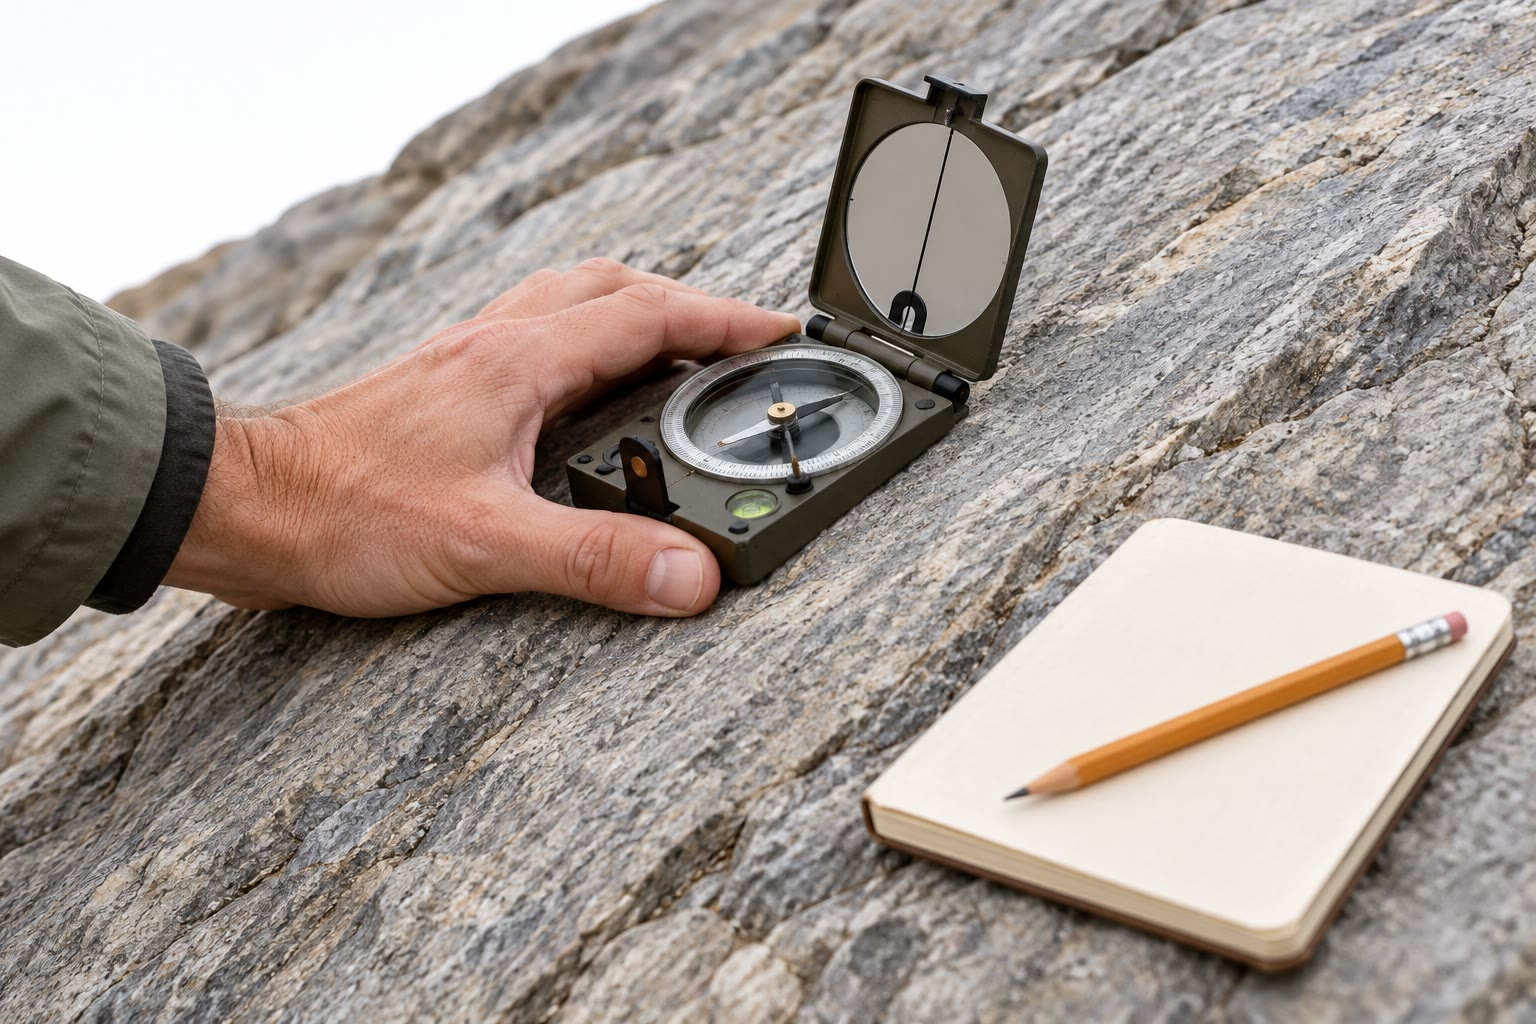
\includegraphics[width=\linewidth]{images/book5/ai/b3-compass-clinometer.jpg}

{\scriptsize بوصلة-مقياس الميل موضوعة على سطح صخري مائل، مع
دفتر ميداني (رسم توضيحي مولَّد بالذكاء الاصطناعي).}
\end{minipage}
\end{inthefield}

\section{التمارين}

\begin{exercise}[$\star$]\label{exo:b3:structural-analysis:1}
احسب الاتجاهَ والغوصَ لقطبِ المستوى $040/30$ (اتجاهَ الانحدار،
الانحدار). أوجد وضعيةَ المستوى الذي يتّجه قطبُه نحو \ang{315} ويغوص
\ang{20}.
\end{exercise}

\begin{exercise}[$\star$]\label{exo:b3:structural-analysis:2}
خطٌّ يغوص بزاوية \ang{30}. على أيّ بُعدٍ من المركز يُرسم
على \omterm{def:b3:structural-analysis:stereo}{الشبكة متساوية الزوايا} وعلى الشبكة متساوية المساحات، وكلتاهما نصف قطرها \qty{10}{cm}؟
\end{exercise}

\begin{exercise}[$\star$]\label{exo:b3:structural-analysis:3}
لأجنحة الطية وضعيتان هما $090/30$ و$270/30$. احسب
الزاويةَ بين قطبيهما بالضرب النقطي للعموديات، وزاويةَ الأجنحة
وصنفَ الطية.
\end{exercise}

\begin{exercise}[$\star$]\label{exo:b3:structural-analysis:4}
يحمل الصدع $090/60$ خدوشًا زاويةُ انزلاقها \ang{-45}. وبمتجهة الامتداد
$\vec s = (0, 1, 0)$ ومتجهة الانحدار نحو الأسفل $\vec d$ للمستوى، فإنّ
انزلاقَ الجدار المعلّق هو $\vec u = \cos r\,\vec s - \sin r\,\vec d$. احسب
$\vec d$، و$\vec u$، والاتجاه والغوص للانزلاق. سمِّ الصدعَ.
\end{exercise}

\begin{exercise}[$\star\star$]\label{exo:b3:structural-analysis:5}
لأجنحة الطية وضعيتان هما $060/40$ و$250/30$. احسب
الاتجاهَ والغوصَ لمحور الطية، وزاويةَ الأجنحة.
\end{exercise}

\begin{exercise}[$\star\star$]\label{exo:b3:structural-analysis:6}
احسب الكسرَ من مساحة الشبكة الواقع داخل دائرةِ
الخطوطِ التي تغوص بأكثر من \ang{60}، على الشبكة متساوية المساحات وعلى \omterm{def:b3:structural-analysis:stereo}{الشبكة متساوية الزوايا}،
والكسرَ من اتجاهات نصف الكرة السفلي التي تغوص بأكثر
من \ang{60}. أيُّ الشبكتين يُستعمل لعدّ الأقطاب؟
\end{exercise}

\begin{exercise}[$\star\star$]\label{exo:b3:structural-analysis:7}
تقع ثلاثة أقطاب في المستوى الشاقولي الممتدّ شرق--غرب، على زوايا \ang{-20} و$0$
و\ang{20} عن الشاقولي: $\vec p = (\sin a, 0, -\cos a)$. احسب
موتّر توجّهها، وقيمها الذاتية ومتجهاتها الذاتية، \omterm{def:b3:structural-analysis:pi}{ومحور بيتا}. لماذا
تكون أصغرُ قيمة ذاتية صفرًا تمامًا؟
\end{exercise}

\begin{exercise}[$\star\star$]\label{exo:b3:structural-analysis:8}
ضع على مخطط فلين الإهليلجيَّ $X : Y : Z = 3 : 1.5 : 1$، ثم
الإهليلجيَّ ذا الحجم الثابت حيث $X = 1.8$ و$Y = 1.1$. احسب $k$ لكلٍّ
منهما، وسمِّ الانفعال.
\end{exercise}

\begin{exercise}[$\star\star$]\label{exo:b3:structural-analysis:9}
في مقطعٍ يُقطع موازيًا للمطّ، تكون الأويدات المستديرة في الأصل
قطوعًا ناقصةً نسبةُ محوريها $2.25$، جميعُها متوازية، ومساحةُ كلٍّ منها
لم تتغيّر. احسب المطّاتِ الرئيسيةَ والاستطالةَ على طول المحور الطويل
المحور الطويل. قبل الانفعال لم تكن مراكزُ الأويدات أقربَ إلى بعضها من
\qty{0.4}{mm}: أعطِ نصفَي المحورين للفراغ الخالي في مخطط فراي.
\end{exercise}

\begin{exercise}[$\star\star\star$]\label{exo:b3:structural-analysis:10}
عند $\theta = \ang{60}$ عن نظير السمت، احسب المطّ على طول نصف القطر،
$\mathrm dr/(R\,\mathrm d\theta)$، وحول الدائرة $r/(R\sin\theta)$،
لكلا الإسقاطين. تحقّق من المبرهنة على الإسقاطات، وأعطِ نسبةَ
محوري البيضاوي الذي تحوّل إليه الشبكةُ متساوية المساحات دائرةً صغيرةً
جدًّا هناك.
\end{exercise}

\begin{exercise}[$\star\star\star$]\label{exo:b3:structural-analysis:11}
في نظامٍ انزياحيّ، يكون $\sigma_1$ أفقيًّا باتجاه \ang{000}،
و$\sigma_3$ أفقيٌّ باتجاه \ang{090}، و$\sigma_2$ شاقوليّ. صدعٌ
شاقوليّ امتداده \ang{020}. دون حساب $\vec\tau$، بيّن أنّ انزلاقه
أفقيٌّ مهما كانت $\Phi$. ثم احسب $-\vec\tau$ عند $\Phi = 0.4$ مع
العمودي على المستوى $\vec n = (\cos\ang{20}, -\sin\ang{20}, 0)$، وأعطِ
جهةَ الانزلاق.
\end{exercise}

\begin{exercise}[$\star\star\star$]\label{exo:b3:structural-analysis:12}
يقطع مقطعٌ طولُه \qty{20}{km} سلسلةً من طيّات الانفصال. أفقان يفصل بينهما
\qty{1.0}{km}، ويعلو كلٌّ منهما مستواه الأصلي بمساحتَيْهما
\qty{6.0}{km^2} (السفلي) و\qty{7.5}{km^2} (العلوي). احسب التقصير،
عمقَ الانفصال تحت الأفق السفلي، والطولَ الأصلي
للمقطع، ونسبةَ تغيّر طوله.
\end{exercise}

\section{مسألة: طيّات وصدوع تلال فاردن}

\begin{problem}[{مسألة نهاية الأسبوع --- محور طيّة وإجهاد مجموعة الصدوع
وترميم المقطع، في منطقة متخيَّلة}]
\label{pb:b3:structural-analysis:1}
% values: calc/ch08.py; figdata/bachelor-3/stereonet.py (data invented from region.py)
في تلال فاردن، المنطقة المتخيَّلة للسلسلة، يرقد غطاء ميزوزوي على
أساسٍ من الشيست والغرانيت. طُويَ الغطاء إلى الطية المحدبة والطية المقعرة
القائمتين بأجنحة مستقيمة، ثم قطعه صدع عادي. قاس جيولوجي
اثني عشر مستوى تطبّقيًا على أجنحة الطية المحدبة
(اتجاه الانحدار/الانحدار، بالدرجات):

\begin{center}
\small
\begin{tabular}{l|cccccc}
\hline
الجناح الشرقي & 075/13 & 084/11 & 089/13 & 079/14 & 086/12 & 072/11 \\
الجناح الغربي & 283/11 & 272/13 & 281/14 & 288/10 & 276/13 & 274/12 \\
\hline
\end{tabular}
\end{center}

مجاميع المتجهات العمودية الواحدية الصاعدة للقراءات الست في كل جناح هي
$\vec S_E = (1.2583, 0.2017, 5.8604)$ و$\vec S_W = (-1.2445, 0.1886,
5.8636)$ (الشرق، الشمال، الأعلى). وتحمل خمسة صدوع خدوشًا انزلاقية (اتجاه الانحدار/الانحدار،
زاوية انزلاق الجدار المعلّق): $120/60/{-90}$ (الصدع الرئيسي)، $150/55/{-76}$،
$090/65/{-108}$، $200/70/{-78}$ و$060/50/{-105}$. للصدع الرئيسي
رمية مقدارها \qty{200}{m}. ويبعد محورا الطية المحدبة والطية المقعرة أحدهما عن الآخر \qty{4}{km}،
بحيث تتكرّر الطيّات كل \qty{8}{km} من الشرق إلى الغرب.

\medskip\noindent\textbf{الجزء الأول --- الأقطاب \omterm{def:b3:structural-analysis:pi}{ومحور بيتا}.}
\begin{enumerate}
  \item أعطِ اتجاه \omterm{def:b3:structural-analysis:stereo}{القطب} وغوصه للقراءة $075/13$،
        ووبُعده عن مركز الشبكة متساوية المساحات ذات نصف القطر
        \qty{10}{cm}.
  \item احسب المتجهة العمودية الواحدية الصاعدة للقراءة $075/13$، ثم
        وتحقّق من مقدارها بالمقارنة مع $\vec S_E$.
  \item احسب الوضعية المتوسطة لكل جناح من $\vec S_E$ و$\vec S_W$،
        وأطوال المحصّلة المتوسطة، والانتشار الجذري لمتوسط المربعات للقراءات
        حول متوسطاتها.
  \item احسب $\vec S_E\times\vec S_W$، واتجاه
        وغوص \omterm{def:b3:structural-analysis:pi}{محور بيتا}.
  \item احسب الزاوية بين العموديين المتوسطين، وزاوية الأجنحة،
        وصنّف الطية.
  \item يحتوي المستوى المحوري لهذه الطية المتماثلة على \omterm{def:b3:structural-analysis:pi}{محور بيتا}، وهو
        عمودي على $\vec m_E - \vec m_W$، فرق المتجهات
        العمودية الواحدية المتوسطة. أعطِ وضعيته؛ هل الطية قائمة؟
  \item أعطِ وضعية حزام $\pi$، وبيّن لماذا تقع الأقطاب
        عليه.
\end{enumerate}

\medskip\noindent\textbf{الجزء الثاني --- \omterm{def:b3:structural-analysis:orientation-tensor}{موتّر التوجّه}.}
\omterm{def:b3:structural-analysis:orientation-tensor}{موتّر التوجّه} للأقطاب الاثني عشر هو
\[
  T = \begin{pmatrix} 0.04400 & 0.00035 & 0.00109\\ 0.00035 & 0.00144 & 0.03179\\
  0.00109 & 0.03179 & 0.95456 \end{pmatrix},
\],
مع القيم الذاتية $0.95562$، $0.04400$ و$0.00038$.
\begin{enumerate}[resume]
  \item تحقّق من أنّ أثر $T$ يساوي 1. ولتكن $\vec b = (0.0053, -0.9994,
        0.0333)$ المتجهة الواحدية على طول $\vec S_E\times\vec S_W$، احسب
        $\vec b^{\mathsf T}T\vec b$. ماذا تقول النتيجة عن $\vec b$؟
  \item احسب الزاوية الجذرية لمتوسط المربعات بين الأقطاب والحزام.
  \item فسّر قيمة $\lambda_2$ انطلاقًا من انحدارات الأجنحة.
  \item هل الطية أسطوانية ضمن دقّة القراءات؟
  \item يتحدّد غوص \omterm{def:b3:structural-analysis:pi}{محور بيتا} بالميل الشمالي--الجنوبي للحزام، الذي يسهم فيه
        كل قطب بالتشتّت الموجود في السؤال 9.
        قدّر الخطأ المعياري للغوص.
\end{enumerate}

\medskip\noindent\textbf{الجزء الثالث --- \omterm{def:b3:structural-analysis:palaeostress}{الإجهاد القديم}.}
\begin{enumerate}[resume]
  \item ما نوع الصدع الرئيسي؟ وفق أندرسون، أعطِ
        اتجاهات $\sigma_1$، $\sigma_2$ و$\sigma_3$.
  \item بيّن، باستعمال مبرهنة اتجاه الانزلاق، أنّ الصدع الرئيسي
        ينزلق انزلاقًا مستقيمًا وفق انحداره مهما تكن قيمة $\Phi$. ماذا يخبرنا
        ذلك عن $\Phi$؟
  \item بالنسبة إلى الصدع $150/55$، احسب $\vec n$ ومركبتيه $n_1 =
        \vec n\cdot\vec e_1$ و$n_2 = \vec n\cdot\vec e_2$، حيث $\vec e_1$
        رأسي و$\vec e_2$ أفقي باتجاه \ang{030}.
  \item يعطي انزلاقه $\vec w = \vec n\times\vec u = (0.771, 0.605, 0.198)$.
        احسب $\Phi$.
  \item تعطي الصدوع الصغيرة الثلاثة الأخرى $\Phi = 0.294$، $0.301$
        و$0.306$. أعطِ المتوسط، وبيّن مصدر التشتّت.
  \item ماذا يقول $\Phi = 0.3$ عن $\sigma_2$؟
  \item احسب محوري P وT للصدع الرئيسي (على زاوية \ang{45} من
        المستوى، في مستوى انحداره)، وقارنهما مع $\sigma_1$
        و$\sigma_3$.
\end{enumerate}

\medskip\noindent\textbf{الجزء الرابع --- ترميم مقطع شرق--غرب.}
\begin{enumerate}[resume]
  \item احسب الانحدار الظاهري للجناح الشرقي، $080.9/12.3$، على مقطع
        شرق--غرب.
  \item بأخذ أجنحة الطيّة عند \ang{12} على المقطع، احسب الطول المرمَّم لموجة طيّة
        واحدة، والتقصير، والتغيّر النسبي
        في الطول.
  \item احسب ارتفاع قمّة الطية المحدبة فوق الطيات المقعّرة، والمساحة
        الزائدة لموجة واحدة، بافتراض أنّ الطيات المقعّرة بقيت
        عند مستواها الأصلي.
  \item احسب عمق الانفصال أسفل الطبقة المطوية. هل يمكن أن تكون الطيّات
        منفصلة عند قاعدة الغطاء، على بُعد بضع مئات من الأمتار
        تحت السطح؟
  \item احسب الإزاحة الأفقية والانزلاق للصدع الرئيسي على مقطع
        باتجاه \ang{120}.
  \item على المقطع شرق--غرب، احسب الانحدار الظاهري للصدع،
        وإزاحته الأفقية الظاهرية. أيّ مقطع ينبغي ترميمه؟
  \item بأيّ ترتيب يُرمَّم الصدع والطيّات، وأين
        تُوضع خطوط التثبيت؟
  \item ما غوص محور طيّة فاردن، كما يُستخلص من
        القراءات الاثنتي عشرة؟
\end{enumerate}
\end{problem}
